\chapter{Subpatterns and Yielding}\indexmain{subpatterns}
\label{cha:sub}

After the introduction of the nested patterns in chapter \ref{cha:nested} we will now have a look at the subpatterns, with the split into subpattern declaration plus subpattern entity declaration and subrule declaration plus usage, the other means to greatly enhances the flexibility and expressiveness of pattern matching and rewriting.

%%%%%%%%%%%%%%%%%%%%%%%%%%%%%%%%%%%%%%%%%%%%%%%%%%%%%%%%%%%%%%%%%%%%%%%%%%%%%%%%%%%%%%%%%%%%%%%%
\section{Subpattern Declaration and Subpattern Entity Declaration}
\indexmain{subpattern}\label{sec:subpattern}

Subpatterns were introduced to factor out a common recurring pattern -- a shape -- into a named subpattern type, ready to be reused at points the pattern should get matched.
The common recurring pattern is specified in a subpattern declaration and used by a subpattern entity declaration.

\begin{rail}  
  SubpatternDeclaration: 
    'pattern' IdentDecl Parameters? (('modify'|'replace') Parameters)? \\
	lbrace SubpatternBody rbrace ;
  SubpatternBody: (PatternStatement+) SubpatternRewriting?;
\end{rail}\ixkeyw{pattern}\ixkeyw{modify}\ixkeyw{replace}\ixnterm{SubpatternDeclaration}\ixnterm{SubpatternBody}\label{subpatterndecl}\indexmain{subpattern declaration}

Subpattern declarations define a subpattern type denoting the specified shape in the global namespace;
the parameters specify some context elements the pattern may refer to, but which are not part of the pattern itself. 
So they are only syntactically the same as test/rule-parameters (which are members of the pattern part).
A further difference is the lack of \emph{ReturnTypes}; they are not actions, just a helper in constructing complex patterns.
In order to get values out they employ the language construct of def entities which are yielded to (cf. \ref{sec:localvarorderedevalyield} later in this chapter).
Subpatterns can receive additional rewrite parameters, in addition to the pattern parameters, in contrast to the actions; they can be used to hand in nodes which are created in the rewrite part of the action or subpattern which contains the subpattern entity.
(The nested body will be explained in Section~\ref{sec:subrule}.)

\begin{rail}  
  SubpatternEntityDeclaration: 
    Ident ':' SubpatternType '(' ((Ident|Expression) * ',') ')' ';' ;
\end{rail}\ixnterm{SubpatternEntityDeclaration}\indexmain{subpattern entity declaration}

Subpattern entity declarations instantiate an entity of the subpattern type (i.e. specified shape), which means the subpattern must get matched for the matching of the enclosing pattern to succeed.
The arguments given are bound to the corresponding parameters of the subpattern.
If you prefer a syntactical point of view, you may see the subpattern entity as a placeholder, which gets substituted in place by the textual body of the subpattern declaration under renaming of the parameters to the arguments.
If you prefer an operational point of view, you may see the subpattern entity as a call to the matcher routine searching for the specified pattern from the given arguments on (constructing a match piece, which is the base for rewriting of that part).

%TODO:remove
%Termersetzung mit Termen die Graphen beschreiben.
%Mehrelementige Graphsprachen als Zwischenschritt zu den rekursiven bereits mit alternative... eingef�hrt -- dort auch so erkl�rt, wirklich eingef�hrt? vor rekursiv trotzdem noch ein  Zwischenschritt: pattern mit alternative, statt action mit alternative

\begin{example}
  \begin{grgen}
pattern TwoParameters(mp:Method)
{
  mp <-- :Variable;
  mp <-- :Variable;
}
test methodAndFurther
{
  m:Method <-- n:Name;
  tp:TwoParameters(m);
}
  \end{grgen}

  In the given example a subpattern \texttt{TwoParameters} is declared, connecting the context element \texttt{mp} via two edges to two variable nodes.
  The test \texttt{methodAndFurther} is using the subpattern via the declaration of the entity \texttt{tp} of type \texttt{TwoParameters}, binding the context element to its local node \texttt{m}.
  The resulting test after subpattern derivation is equivalent to the test \texttt{methodWithTwoParameters}.

  \begin{grgen}
test methodWithTwoParameters
{
  m:Method <-- n:Name;
  m <-- :Variable;
  m <-- :Variable;
}
  \end{grgen}
\end{example}

%-----------------------------------------------------------------------------------------------
\subsection{Recursive Patterns}\indexmain{recursive pattern}\indexmain{structural recursion}

Subpatterns can be combined with alternative patterns or the cardinality patterns into recursive subpatterns, i.e. subpatterns which may contain themselves.
Subpatterns containing themselves alone -- directly or indirectly -- would never yield a match as an infinite pattern can't be found in a limited graph.

\begin{example}\label{exiterpath}
  \begin{grgen}
test iteratedPath
{
  root:Assign;
  negative { --> root; }
  :IteratedPath(root); // match iterated path = assignment list
}

pattern IteratedPath(prev:Node)
{
  optional { // nothing or a linked assignment and again a list
    prev --> a:Assign; // assignment node 
    :IteratedPath(a); // next one, plz
  }
}
  \end{grgen}
  
The code above searches an \indexed{iterated path} from the root node on, here an assignment list. 
The iterated \indexed{path} with the optional is equivalent to the code below. Note the negative which ensures you get a longest match -- without it the empty case may be chosen lazily just in the beginning.
Please note that if you only need to check for the existence of such a simple iterated path you can use the \texttt{reachable} functions introduced in \ref{transitiveneighbour}.

  \begin{grgen}
pattern IteratedPath(prev:Node)
{
  alternative {
    Empty {
      negative {
        prev --> a:Assign;
      }
    }
    Further {
      prev --> a:Assign;
      :IteratedPath(a);
    }
  }
}
  \end{grgen}

The code below searches an iterated path like the code above, just that it stops when a maximum length is reached.
The \indexed{bounded iterated path} is realized by 
calling a pattern with the requested maximum depth,
counting the depth parameter down with each recursion step,
until the limit checked by a condition is reached.
The \texttt{boundedReachable} functions introduced in \ref{transitiveneighbourbounded} should be prefered in a simple case like this.

  \begin{grgen}
test boundedIteratedPath(root:Assign)
{
  :BoundedIteratedPath(root, 3); // match iterated path of depth 3
}

pattern BoundedIteratedPath(prev:Node, var depth:int)
{
  optional { // nothing or a linked assignment and again a list
    prev --> a:Assign; // assignment node 
    :IteratedPath(a, depth-1); // next one, plz
    if{ depth >= 1; } // stop when we have reached max depth
  }
}
  \end{grgen}
\end{example}

\begin{example}
  \begin{grgen}
rule removeMiddleAssignment
{
  a1:Assign --> a2:Assign --> a3:Assign;
  independent {
    :IteratedPath(a1,a3)
  }
  
  replace {
    a1; a3;
  }
}

pattern IteratedPath(begin:Assign, end:Assign)
{
  alternative { // an iterated path from begin to end is either
    Found { // the begin assignment directly linked to the end assignment (base case)
      begin --> end;
    }
    Further { // or an iterated path from the node after begin to end (recursive case)
      begin --> intermediate:Assign;
      :IteratedPath(intermediate, end);
    }
  }
}
  \end{grgen}

This is once more a fabricated example, for an iterated path from a source node to a distinctive target node, and an example for the interplay of subpatterns and positive application conditions to check complex conditions independent from the pattern already matched.
Here, three nodes \texttt{a1},\texttt{a2},\texttt{a3} of type \texttt{Assign} forming a list connected by edges are searched, and if found, \texttt{a2} gets deleted, but only if there is an iterated path of directed edges from \texttt{a1} to \texttt{a3}.
The path may contain the host graph node matched to \texttt{a2} again.
Without the \texttt{independent} this would not be possible, as all pattern elements -- including the ones originating from subpatterns -- get matched isomorphically. 
The same path specified in the pattern of the rule -- not in the independent -- would not get matched if it would go through the host graph node matched to b, as it is locked by the isomorphy constraint.
Again, the \texttt{reachable} functions introduced in \ref{transitiveneighbour} are the better choice here.
They always match independently from the patterns (so when you need locking, you cannot employ them), can be used directly, and are implemented (more) efficiently. 
\end{example}

With recursive subpatterns you can already capture neatly structures extending into depth (as iterated paths)
and also structures extending into breadth (as forking patterns, although the cardinality statements are often much better suited to this task).
But combined with an iterated block, you may even match structures extending into breadth and depth,
like e.g. an inheritance hierarchy of classes in our example domain of program graphs, see example \ref{exsptree}, i.e. you can match a \indexed{spanning tree} in the graph.
This gives you a very powerful and flexible notation to capture large, complex patterns
built up in a structured way from simple, connected pieces (as e.g. abstract syntax trees of programming languages). 

\begin{note}
If you are working with hierarchic structures like that, 
you might be interested in the capabilities of GrShell/yComp for nested layout
as described and shown in \ref{sub:visual}/\ref{note:visual}).
\end{note}

\begin{example}\label{exsptree}
  \begin{grgen}
pattern SpanningTree(root:Class)
{
  iterated {
    root <-:extending- next:Class;
    :SpanningTree(next);
  }
}
  \end{grgen}
\end{example}


%%%%%%%%%%%%%%%%%%%%%%%%%%%%%%%%%%%%%%%%%%%%%%%%%%%%%%%%%%%%%%%%%%%%%%%%%%%%%%%%%%%%%%%%%%%%%%%%
\section{Subpattern Rewriting}
\indexmain{subrule}\label{sec:subrule}

Alongside the separation into subpattern declaration and subpattern entity declaration, 
subpattern rewriting is separated into a nested rewrite specification given within the subpattern declaration defining how the rewrite looks like 
and a subpattern rewrite application given within the rewrite part of the pattern containing the subpattern entity declaration requesting the rewrite to be actually applied.

\begin{rail}  
  SubpatternRewriting: ('replace' | 'modify') lbrace (()+RewriteStatement) rbrace;
\end{rail}\ixnterm{SubpatternRewriting}\ixkeyw{replace}\ixkeyw{modify}

The subpattern rewriting specifications within the subpattern declaration looks like a nested rewriting specification,
but additionally there may be rewrite parameters given in the subpattern header (cf. \ref{subpatterndecl}) which can be referenced in the rewrite body.
(Most elements can be handed in with normal parameters, but elements created in the rewrite part of the user of the subpattern can only be handed in at rewrite time.) 

\begin{rail}  
  SubpatternRewriteApplication: 
    Ident '(' (Ident * ',') ')' ';' |
    SubpatternOccurence |
    SubpatternExecEmit
	;
\end{rail}\ixnterm{SubpatternRewriteApplication}

\noindent The \emph{SubpatternRewriteApplication} is part of the \emph{RewriteStatement} already introduced (cf. \ref{replstmt}).
The subpattern rewrite application is given within the rewrite part of the pattern containing the subpattern entity declaration,
in call notation on the declared subpattern identifier.
It causes the rewrite part of the subpattern to get used; if you leave it out, the subpattern is simply kept untouched.
The \emph{SubpatternOccurence} is explained in the next subsection \ref{sub:delpressub}.
The \emph{SubpatternExecEmit} is explained in chapter \ref{cha:imperativeandstate}.

\begin{example}
This is an example for a subpattern rewrite application.

  \begin{grgen}
pattern TwoParametersAddDelete(mp:Method)
{
  mp <-- v1:Variable;
  mp <-- :Variable;

  modify {
    delete(v1);
    mp <-- :Variable;
  }
}
rule methodAndFurtherAddDelete
{
  m:Method <-- n:Name;
  tp:TwoParametersAddDelete(m);

  modify {
    tp(); // trigger rewriting of the TwoParametersAddDelete instance
  }
}
  \end{grgen}
\end{example}


\begin{example}
This is another example for a subpattern rewrite application,
reversing the direction of the edges on an iterated path.

  \begin{grgen}
pattern IteratedPathReverse(prev:Node)
{
  optional {
    prev --> next:Node;
    ipr:IteratedPathReverse(next);
    
    replace {
      prev <-- next;
      ipr();
    }
  }

  replace {
  }
}
  \end{grgen}
\end{example}

\begin{example}
This is an example for rewrite parameters, connecting every node on an iterated path to a common node (i.e. the local rewrite graph to the containing rewrite graph).
It can't be simulated by subpattern parameters which get defined at matching time because the common element is only created later on, at rewrite time.

  \begin{grgen}
pattern ChainFromToReverseToCommon(from:Node, to:Node) replace(common:Node)
{
  alternative {
    rec {
      from --> intermediate:Node;
      cftrtc:ChainFromToReverseToCommon(intermediate, to);

      replace {
        from <-- intermediate;
        from --> common;
        cftrtc(common);
      }
    }
    base {
      from --> to;

      replace {
        from <-- to;
        from --> common;
        to --> common;
      }
    }
  }

  replace {
    from; to;
  }
}
  \end{grgen}

  \begin{grgen}  
rule chainFromToReverseToCommon()
{
  from:Node; to:Node;
  cftrtc:ChainFromToReverseToCommon(from, to);

  modify {
    common:Node;
    cftrtc(common);
  }
}
  \end{grgen}
\end{example}

%-----------------------------------------------------------------------------------------------
\subsection{Deletion and Preservation of Subpatterns}\label{sub:delpressub}

In addition to the fine-grain dependent rewrite, subpatterns may get deleted or kept as a whole.

\begin{rail}  
  SubpatternOccurence: 
    Ident ';' |
    'delete' '(' (Ident + ',') ')' ';';
\end{rail}\ixkeyw{SubpatternOccurence}\ixkeyw{delete}

In modify mode, they are kept by default, but deleted if the name of the declared subpattern entity is mentioned within a delete statement.
In replace mode, they are deleted by default, but kept if the name of the declared subpattern entity is mentioned (using occurrence, same as with nodes or edges).

\begin{example}
  \begin{grgen}
rule R {
  m1:Method; m2:Method;
  tp1:TwoParameters(m1);
  tp2:TwoParameters(m2);

  replace {
    tp1; // is kept
    // tp2 not included here - will be deleted
    // tp1(); or tp2(); -- would apply dependent replacement
    m1; m2;
  }
}
  \end{grgen}
\end{example}

\begin{note}
You may even give a SubpatternEntityDeclaration within a rewrite part which causes the subpattern to be created; 
but this employment has several issues which can only be overcome by introducing explicit creation-only subpatterns
-- so you better only use it if you think it should obviously work (examples for the issues are alternatives -- which case to instantiate? -- and abstract node or edge types -- what concrete type to choose?). 

  \begin{grgen}
pattern ForCreationOnly(mp:Method)
{
  // some complex pattern you want to instantiate several times 
  // connecting it to the mp handed in
}
rule createSubpattern
{
  m:Method;
  
  modify {
    :ForCreationOnly(m); // instantiate pattern ForCreationOnly
  }
}
  \end{grgen}
\end{note}


%%%%%%%%%%%%%%%%%%%%%%%%%%%%%%%%%%%%%%%%%%%%%%%%%%%%%%%%%%%%%%%%%%%%%%%%%%%%%%%%%%%%%%%%%%%%%%%%
\section{Local Variables, Ordered Evaluation, and Yielding Outwards} \label{sec:localvarorderedevalyield}\indexmain{local variable}\indexmainsee{evalhere}{ordered evaluation}\indexmain{yielding outwards}

\subsection*{Local Variables and Ordered Evaluation} 
Sometimes attribute evaluation becomes easier with temporary variables;
such local variables can be introduced on a right hand side employing the known variable syntax \texttt{var name:type}, prefixed with the \texttt{def}\indexmain{def} keyword.
From then on they can be read and assigned to in eval statements of the RHS, or used as variable parameters in subpattern rewrite calls.
In addition, on their introduction an initializing expression may be given.

\begin{example}
  \begin{grgen}
rule R {
  n1:N; n2:N; n3:N; n4:N; n5:N;
  
  modify {
    def var mean:double = (n1.v + n2.v + n3.v + n4.v + n5.v)/5;
    eval {
    	n1.variance = (n1.v - mean)*(n1.v - mean); 
    	n2.variance = (n2.v - mean)*(n2.v - mean); 
    	n3.variance = (n3.v - mean)*(n3.v - mean); 
    	n4.variance = (n4.v - mean)*(n4.v - mean); 
    	n5.variance = (n5.v - mean)*(n5.v - mean); 
    }
  }
}
  \end{grgen}
\end{example}


Normally the rewrite order is as given in table \ref{table:executionorderrewriting}:
\begin{table}[htbp]
  \centering
  \begin{tabularx}{\linewidth}{|l|X|} \hline
    \texttt{ 1. } & \texttt{ Extract elements needed from match } \\
    \texttt{ 2. } & \texttt{ Create new nodes } \\
    \texttt{ 3. } & \texttt{ Call rewrite code of used subpatterns} \emph{and more...} \\ 
	  \texttt{ 4. } & \texttt{ Call rewrite code of nested iterateds } \\
    \texttt{ 5. } & \texttt{ Call rewrite code of nested alternatives } \\
    \texttt{ 6. } & \texttt{ Redirect edges } \\  
    \texttt{ 7. } & \texttt{ Retype (and merge) nodes } \\  
    \texttt{ 8. } & \texttt{ Create new edges } \\
    \texttt{ 9. } & \texttt{ Retype edges } \\  
    \texttt{ 10. } & \texttt{ Create subpatterns } \\
    \texttt{ 11. } & \texttt{ Attribute reevaluation } \\
    \texttt{ 12. } & \texttt{ Remove edges } \\ 
	  \texttt{ 13. } & \texttt{ Remove nodes } \\
    \texttt{ 14. } & \texttt{ Remove subpatterns } \\
    \texttt{ 15. } & \texttt{ Emit / Exec } \\  
    \texttt{ 16. } & \texttt{ Return } \\ \hline
	\end{tabularx}
	{\small \emph{and more...} at \texttt{3.} are \texttt{evalhere}, \texttt{emithere}, \texttt{alternative} Name, \texttt{iterated} Name}
  \caption{Execution order rewriting}
  \label{table:executionorderrewriting}
\end{table}

So first the subpatterns rewrites, then the iterated rewrites, then the alternative rewrites are executed, and finally the local eval statements (computations).
This might be sufficient in some cases, but in other cases when you want to compute an attributation over a tree/a graph, you want to have local computations influenced by attributes in nested/called children or its siblings, and attributes in nested/called children influenced by its parents or siblings.
So we need a language device which allows us to intermingle attribute computations in between the rewrite part executions of nested patterns and subpattern rewrite calls.
And a language device which allows us to give the execution oder of the alternative and iterated statements relative to the subpattern rewrite calls and attribute evaluations.

To achieve attribute evaluation in a defined order in between the subpattern rewrite calls, we use ordered evaluation statements, introduced with the keyword \texttt{evalhere}; 
they get executed in the order in which they are given syntactically
(a further statement executed in order is \texttt{emithere}, introduced in \ref{sec:deferredexecemithere}).

To achieve iterated/alternative execution in order, we allow names to be given to nested patterns, and reuse this name in a nested pattern rewrite order specification.
Naming nested patterns is done with the following syntax, as the already introduced syntax remains valid, on aggregate we extend the nested patterns with optional names to form \indexed{named nested pattern}.

\begin{rail}  
  NamedNestedPattern: 
    ('negative' | 'independent') IdentDecl lbrace etc rbrace;
    ('iterated' | 'multiple' | 'optional') IdentDecl etc rbrace;
    'alternative' IdentDecl lbrace etc rbrace;
\end{rail}

Alternatives and iterateds named this way can then be referenced in the rewrite part with an alternative rewrite order specification or an iterated rewrite order specification.

\begin{rail}  
  CardinalityRewriteUsage: 
    ('iterated' | 'multiple' | 'optional') Ident ';';
  AlternativeRewriteUsage: 
    'alternative' Ident ';';
\end{rail}

What we've seen so far is applied in the following example.
A \texttt{yield} prefix is needed whenever a \texttt{def} variable is written to (as  assignment target as well as a subpattern output argument). 

\begin{example}
  \begin{grgen}
rule R {
  iterated foo { .; modify { ..read i.. } }
  alternative bar { case { modify { ..read i.. } } } 
  sub1:Subpattern1();
  sub2:Subpattern2();

  modify {
    def var i:int = 0; // initializes i to 0
    evalhere { yield i = i + 1; } // afterwards i==1
    sub1(i); // input 1 to subpattern rewrite
    evalhere { yield i = i + 1; } // afterwards i==2
    iterated foo; // nested iterated reads i==2 
    evalhere { yield i = i + 1; } // afterwards i==3
    alternative bar; // nested alternative reads i==3
    evalhere { yield i = i + 1; } // afterwards i==4
    sub2(i); // input 4 to subpattern rewrite
    evalhere { yield i = i + 1; } // afterwards i==5
    eval { yield j = i + 1; } // assign 6 to j
  }
}
  \end{grgen}
\end{example}

\begin{note}
For rewriting the execution order of the parts can be defined, to allow programming attribute evaluation orders of interest, defining when to descend into which part and defining glueing/local computations in between.
(A depth first run with a defined order in between the siblings, comparable to an LAG/RAG run in compiler construction, but with an explicitly defined sequence of children visits, instead of a temporal succession implicitly induced by the syntactical left-to-right ordering).
In contrast to rewriting, the \emph{matching} order of the pattern parts can \emph{not} be defined, to allow the compiler/the runtime to use the evaluation order it estimates to be the best.
So we can't access attributes from sibling elements, we can only compute attributes top down from local elements or elements handed in on matching, and later on bottom up from local elements or elements bubbling up at match object tree construction.
Top down attribute evaluation operates on the already matched elements and attribute values or the ones received as inputs, which are handed down implicitly into nested patterns or explicitly via subpattern parameters into subpattern instances. (A depth first run too, but without a defined order in between the siblings, comparable to an IAG run in compiler construction for computing inherited attributes during matching while descending).
Bottom up attribute evaluation operates on the matched elements and attribute values locally available or the ones received into def elements yielded implicitly upwards from the nested patterns or explicitly accumulating iterated results or with assigning out parameters of subpatterns. (The same depth first run, but with attributes computed while ascending, comparable to an SAG run in compiler construction for computing synthesized attributes.)
\end{note}

\subsection*{Yielding Outwards During Rewriting}\label{sub:yield} 

Sometimes one needs to bring something matched within a nested or subpattern to an outer pattern containing it (nested patterns) or calling it (subpatterns).
So that one can do there (in the using pattern) operations on it, e.g. attaching a further edge to an end node of a chain matched with recursive patterns (thus modularizing the graph rewrite specification into chain matching patterns and patterns using chains doing things on the chain ends), or summing attributes matched in iterated pattern instances. 

The first thing one needs to bring something outwards is a target in a nesting or calling pattern. 
This is achieved by nodes, edges, and variables declared with the \texttt{def} keyword in a rewrite part, marking them as output entities;
variables were already introduced in previous paragraphs, but in addition to them nodes and edges are allowed, too.
Furthermore subpattern rewrite parameters may be declared as def parameters,
marking them as output parameters.
These elements are then yielded to from within \texttt{eval} or \texttt{evalhere} statements, subpattern rewrite usages, and \texttt{exec} statements.
While the latter will be covered in chapter \ref{cha:imperativeandstate}, the former will be explained in the following.

Yielding is specified by prepending the \texttt{yield}\indexmain{yield} keyword to the entity yielded to,
in an assignment to a variable or a method call on a variable,
inside an \texttt{eval} or \texttt{evalhere}-statement, or a change assignment; 
the target of the assignment may be a node or edge (if declared as output variable).
The yield must be prepended to the argument for a subpattern def rewrite parameter, too.

\begin{example}
  \begin{grgen}
pattern Chain(begin:Node) modify(def end:Node)
{
  alternative {
    Further {
      begin --> intermediate:Node;
      c:Chain(intermediate);
      
      modify {
        c(yield end);
      }
    }
    Done {
      negative {
        begin --> ;
      }
      
      modify {
        eval {
          yield end = begin;
        }
      }
    }
  }
  
  modify { }
}

rule R(begin:Node) : (Node) {
  c:Chain(begin);

  modify {
    def end:Node;
    c(yield end); // end is filled with chain end
    return(end);
  }
}
  \end{grgen}
  First example for RHS yielding: returning the end node of a chain.
\end{example}

\begin{example}
  \begin{grgen}
rule outCount(head:Node) : (int)
{
  iterated {
    head --> .;
    modify {
      eval { yield count = count + 1; }
    }
  }

  modify {
    def var count:int = 0;
    return (count);
  }
}
  \end{grgen}
  Second example for RHS yielding: counting the number of edges matched with an iterated.
\end{example}

\subsection*{Yielding Outwards During Match Object Construction} 

Bubbling up the elements from nested patterns and called patterns during rewriting might be too late or inconvenient.
Luckily it can be done before, at the end pattern matching when the match object tree gets constructed.

As for RHS yielding the targets of the yielding must be nodes, edges, or variables declared with the \texttt{def} keyword prepended, marking them as output entities; but this time in the pattern part.
Furthermore subpattern parameters may be declared as def parameters in the subpattern definition header, marking them as output parameters.

These elements can then be yielded to from within \texttt{eval} statements inside a \texttt{yield} block
(maybe with iterated accumulation) and subpattern usages.
A \texttt{yield} block is a constrained \texttt{eval} block which can be given in the pattern part;
it does not allow to assign to or change non-\texttt{def} variables, or carry out graph-changing commands.
Yielding is specified by prepending the \texttt{yield}\indexmain{yield} keyword to the entity yielded to,
in the assignment or method call.
The \texttt{yield} must be prepended to the argument for a subpattern def parameter, too.

\begin{warning}
A def entity from the pattern part can't be yielded to from the rewrite part, they are constant after matching.
\end{warning}

Let's have a look at two examples for yielding:

\begin{example}
  \begin{grgen}
pattern Chain(begin:Node, def end:Node)
{
	alternative {
		further {
			begin --> next:Node;
			:Chain(next, yield end);
		}
		done {
		  negative {
		    begin --> ;
		  }
			yield {
				yield end = begin;
			}
		}
	}
}

pattern LinkChainTo(begin:Node) modify(n:Node)
{
	alternative {
		further {
			begin --> next:Node;
			o:LinkChainTo(next);

			modify {
			  next --> n;
			  o(n);
			}
		}
		done {
		  negative {
		    begin --> ;
		  }
		  
			modify {
			}
		}
	}

	modify { }
}

rule linkChainEndToStartIndependent(begin:Node) : (Node)
{
	def end:Node;
	
	independent {
		c:Chain(begin, yield end);
	}
  o:LinkChainTo(begin);
  	
	modify {
	  o(end);
		return(end);
	}
}
  \end{grgen}
\end{example}

The first example for LHS yielding follows within an independent a chain piece by piece to some a priori unknown end node, and yields this end node chain piece by chain piece again outwards to the chain start. There it is used as input to another chain (maybe the same chain, maybe overlapping due to the independent), linking all the nodes of this chain to the end node of the former.

When yielding from an iterated pattern there's the problem that each yielding assignment from an iterated instance would overwrite the one def variable from outside the iterated, while one is interested most of the time in some accumulation of the values, e.g. summing integers or concatenating strings.
This can be achieved with a \texttt{for} loop iterating a def variable inside an iterated for all the matches of the iterated pattern referenced by name, allowing to assign to an outside def variable a value computed from the def variable and the value of the iterated def variable.

This is shown in the second example for LHS yielding, summing the integer attribute \texttt{a} of nodes of type \texttt{N} adjacent to a start node, matched with an iterated.

\begin{example}
  \begin{grgen}
test sumOfWeight(start:Node) : (int,int)
{
	def var sum:int = 0;
	def var v:int = 0;
	
	iterated it {
		def var i:int;
		
		start --> n:N; // node class N { a:int; }
		
		yield {
			yield i = n.a;
			yield v = 42; // v is assigned 42 multiple times
		}
	} 

	yield {
		for(i in it)
		{
		  yield sum = sum + i;
		}
	}

	return (sum,v);
}
  \end{grgen}
\end{example}

In case no accumulation is needed but a simple \indexed{count} of the iterated matches is sufficient, one can employ the \texttt{count} operator on an iterated (that must have been named before), as displayed in the following example (the count is only available in a \texttt{yield} or \texttt{eval} block).

\begin{example}
  \begin{grgen}
test countOfEdges(start:Node) : (int)
{
	def var sum:int = 0;
	
	iterated it {
		start -->;
	} 

	yield {
	  yield sum = count(it);
	}

	return (sum);
}
  \end{grgen}
\end{example}

%\pagebreak

%%%%%%%%%%%%%%%%%%%%%%%%%%%%%%%%%%%%%%%%%%%%%%%%%%%%%%%%%%%%%%%%%%%%%%%%%%%%%%%%%%%%%%%%%%%%%%%%
\section{Flow Example, Regular Expression Syntax, and Locking}\indexmainsee{EBNF}{regular expression syntax}\indexmain{regular expression syntax}\label{matchingflow}

Pattern matching and rewriting occurs in two completely distinct passes, separated by the part-pattern matches tree of the combined patterns.
During each pass, input and output parameters may be computed and passed; with explicit passing for subpatterns, and implicit passing for nested patterns (which can directly access the content of their contained pattern).

First the pattern is matched with recursive descent alongside pattern nesting and subpattern calling, employing some helper stacks in addition to the call stack (the pushdown machine is explained in more detail in \ref{sec:generatedcode}).
Matching occurs strictly top-down (or from the outside to the nested inside patterns), first the graphlets of the current pattern are matched, then control descends to the nested and subpatterns.
During matching, input parameters may be passed, esp. forwarding just matched elements or attributes from them; they allow to influence the matching process.

When a complete match is found, while ascending again, unwinding the call stack, output pattern-\texttt{def} parameters are passed bottom-up (or from the inside to the containing outside patterns) with \texttt{yield} blocks and \texttt{yield} assignments within those blocks, or \texttt{yield} bindings of \texttt{def} parameters in a subpattern call.
During this ascent, the part-pattern matches tree is assembled, each match of a pattern contains the matches of its nested patterns and used subpatterns when it is left.

In the rewrite step, the matches tree is visited recursively again, creating the new nodes of the current pattern, then descending to the nested patterns and subpatterns, executing their changes, and after they returned, executing all other changes of the pattern.
During this visit, rewrite input parameters may be passed, for forwarding just created elements (or computed values). 

On ascending again from a pattern, the rewrite-\texttt{def} elements are assigned from \texttt{yield} assignments in the \texttt{eval} blocks, or \texttt{yield} bindings of \texttt{def} rewrite parameters in a subpattern rewrite call.
(Technically, nested patterns are handled like subpatterns, with parameter passing for accessed elements of the containing pattern automatically inserted by the compiler.)

Let's take a look at an example, with Figure \ref{figmatchingparameterflow} depicting the input and output parameter passing during the matching of Example \ref{exmatchingparameterflow}, and Figure \ref{figrewritingparameterflow} depicting the input and output parameter passing during the rewriting of Example \ref{exrewritingparameterflow} (which is an extended version of Example \ref{figmatchingparameterflow}).

\begin{example}
  \begin{grgen}
rule r(a:Node) : (Node, int)
{
	a --> b:Node;
	
	def var i:int;
	optional o {
		a --> . --> c:N;
		yield { yield i = c.i; }
		
		modify {
		}
	}

	def d:Node;
	p:P(b, yield d);
	
	modify {
		b --> u:Node;
		return(d, i);
	}
}

pattern P(n:Node, def rm:Node)
{
	n --> . --> m:Node;
	yield { yield rm = m; }
}
  \end{grgen}
\end{example}\label{exmatchingparameterflow}

\begin{figure}[hptb]
  \centering
  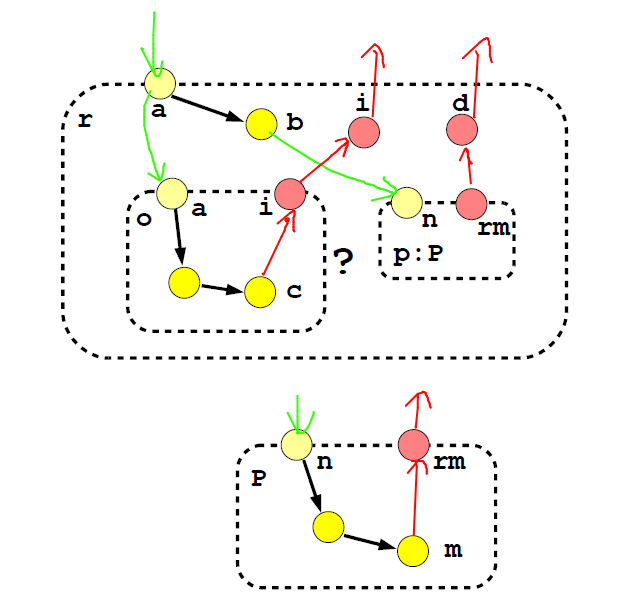
\includegraphics[width=0.61\textwidth]{fig/MatchAndParameterFlowAnnotated}
  \caption{Parameter flow in matching}
  \label{figmatchingparameterflow}
\end{figure}

\begin{example}
  \begin{grgen}
rule r(a:Node) : (Node, int, Node, int) {
	a --> b:Node;
	def var i:int;
	optional o {
		a --> . --> c:N;
		yield {	yield i = c.i; }
		
		modify {
			eval { yield j = i + u.i; }
		}
	}
	def d:Node;
	p:P(b, yield d);
	
	modify {
		def e:Node; def var j:int;
		b --> u:N;
		p(u, yield e);
		return(d, i, e, j);
	}
}
pattern P(n:Node, def rm:Node) modify(k:Node, def x:Node) {
	n --> . --> m:Node;
	yield {	yield rm = m; }
	
	modify {
		m --> k; m --> l:Node;
		eval { yield x = l; }
	}
}
  \end{grgen}
\end{example}\label{exrewritingparameterflow}

\begin{figure}[hptb]
  \centering
  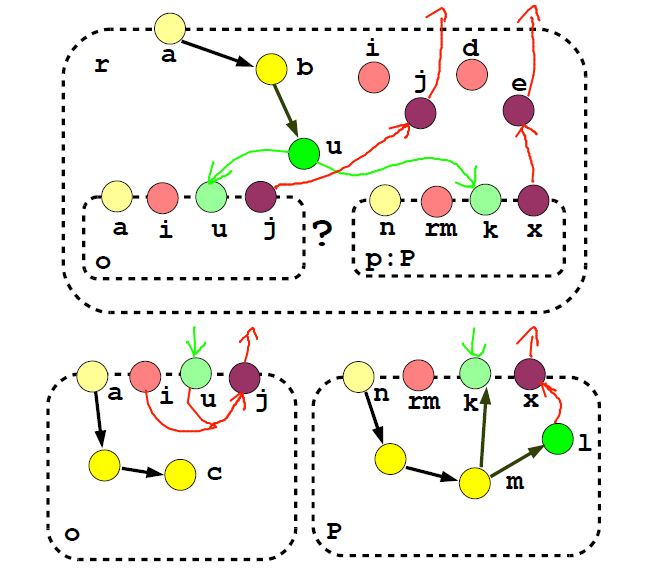
\includegraphics[width=0.63\textwidth]{fig/RewriteAndParameterFlowAnnotated}
  \caption{Parameter flow in rewriting}
  \label{figrewritingparameterflow}
\end{figure}

In Example \ref{exmatchingparameterflow}, a rule \texttt{r} is matched, which contains a nested \texttt{optional} pattern \texttt{o} and uses a subpattern \texttt{P}.
The rule matches from its input node \texttt{a} on a neighbouring node \texttt{b} and hands it in to the subpattern \texttt{p}.
In the optional pattern it matches a two-step neighbouring node \texttt{c} from \texttt{a} on.
The subpattern \texttt{P} matches from its input parameter \texttt{n} on a two-step neighbouring node \texttt{m}.

A \texttt{def} variable \texttt{i} is declared in the pattern, and \texttt{yield} assigned from the optional \texttt{o} an attribute of the \texttt{c} found there.
Another \texttt{def} variable \texttt{d} is declared in the pattern, and assigned from the subpattern call \texttt{p} with a \texttt{yield} parameter passing. 
The two pattern \texttt{def} variables are then \texttt{return}ed out of rule \texttt{r}.
The subpattern \texttt{P} \texttt{yield}s to its output \texttt{def} parameter \texttt{rm} the \texttt{m} found in its body.

In the extended Example \ref{exrewritingparameterflow}, the rewrite part of the rule \texttt{r} creates a node \texttt{u}, links it to \texttt{b}, and hands it in to the subpattern rewrite employment of \texttt{p}.
The rewrite part of subpattern \texttt{P} creates a node \texttt{l} and links it to \texttt{m}.
Additionally, an edge is inserted in between \texttt{m} and the rewrite input parameter \texttt{k}.

A \texttt{def} variable \texttt{j} is declared in the rewrite part of \texttt{r}, and \texttt{yield} assigned from the \texttt{eval} inside the rewrite part of the optional \texttt{o}.
Another \texttt{def} variable \texttt{e} is declared in the rewrite part, and assigned from the subpattern rewrite call \texttt{p}.
The two rewrite-\texttt{def} variables are then \texttt{return}ed out of the rule, in addition to the two pattern-\texttt{def} variables.
The subpattern \texttt{yield}s from its \texttt{eval} part to its output \texttt{def} rewrite parameter \texttt{x} the \texttt{l} just created.

Bottom line: you can flexibly combine patterns with nested and subpatterns, including input and output parameters.
You can pass parameters in during matching alongside matching order. When matching completed, during match-tree building, you can yield elements found in contained patterns out. 
When the rewrite is applied, you can pass parameters in alongside the buildup of the patterns, and yield elements out once more.
But not only are those two passes strictly distinct, but also are the parameter passing directions strictly distinct, first is all input parameter passing carried out during descent, then is all output parameter synthesizing carried out during ascent.


\subsubsection*{Regular Expression Syntax}
In addition to the already introduced syntax for the nested patterns with the keywords 
\texttt{negative}, \texttt{independent}, \texttt{alternative}, \texttt{iterated}, \texttt{multiple} and \texttt{optional},
there is a more lightweight syntax resembling regular expressions available; 
when used together with the subpatterns it yields graph rewrite specifications which look like EBNF-grammars with embedded actions. 
Besides reducing syntactical weight, they offer constructs for matching a pattern a bounded number of times (same notation as the one for the bounded iteration in the sequences).

%Table \ref{keywordregexpsyntax} lists the corresponding (/equivalent) language constructs; 
%Example \ref{introexampleregexp} is a version of the introductory example \ref{introexample} modified to use the new syntax. commented out to get better layout

\begin{table}[htbp]
  \centering
  \begin{tabularx}{\linewidth}{|l|X|} \hline
    \texttt{ iterated \{ P \} } & \texttt{ (P)* } \\
    \texttt{ multiple \{ P \} } & \texttt{ (P)+ } \\
    \texttt{ optional \{ P \} } & \texttt{ (P)? } \\ 
	\texttt{ alternative \{ l1 \{ P1 \} .. lk \{ Pk \} \} } & \texttt{ (P1|..|Pk) } \\
    \texttt{ negative \{ P \} } & \texttt{ $\sim$(P) } \\
    \texttt{ independent \{ P \} } & \texttt{ \&(P)} \\ \hline 
    \texttt{ modify \{ R \} } & \texttt{  \{+ R \} } \\
    \texttt{ replace \{ R \} } & \texttt{ \{- R \} } \\ \hline 
    \texttt{ - } & \texttt{ (P)[k] / (P)[k:l] / (P)[k:*] } \\ \hline 
	\end{tabularx}
  \caption{Map of nested patterns in keyword syntax to regular expression syntax}
  \label{keywordregexpsyntax}
\end{table}

Understanding \GrG-subpatterns may be easier given knowledge about EBNF-grammars when we compare them to those.
We find then that rules resemble grammar axioms, subpatterns resemble nonterminals, and graphlets resemble terminal symbols; nested patterns are similar to EBNF operators, and the rewrite part corresponds to the semantic actions of syntax directed translation.
Negative and independent patterns are used to explicitly check context constraints
(every graphlet as such is already able to match pieces that one would or could classify as context, graph rewriting allows for derivations that are highly adaptable to the surrounding parts).
See \cite{EBNFAGTIVE} for more on this.

  \begin{example}
    \begin{grgen}
test method
{
  m:Method <-- n:Name; // signature of method consisting of name
  ( m <-- :Variable; )* // and 0-n parameters
  
  :AssignmentList(m); // body consisting of a list of assignment statements
}

pattern AssignmentList(prev:Node)
{
  ( // nothing or a linked assignment and again a list
    prev --> a:Assign; // assignment node 
    a -:target-> v:Variable; // which has a variable as target 
    :Expression(a);  // and an expression which defines the left hand side 
    :AssignmentList(a); // next one, plz
  )?
}

pattern Expression(root:Expr)
{
  ( // expression may be a binary expression of an operator and two expresions
      root <-- expr1:Expr;
      :Expression(expr1);
      root <-- expr2:Expr;
      :Expression(expr2);
      root <-- :Operator;
  | // or a unary expression which is a variable (reading it)
      root <-- v:Variable;
  )
}
    \end{grgen}
  \end{example}\label{introexampleregexp}

\subsubsection*{Isomorphy Locking} \label{locking}
When matching a program graph as in the introductory example \ref{ex:proggraph} one might be satisfied with matching a tree structure.
But on other occasions one wants to match \emph{backlinks} and especially the targets of the backlinks, too, 
from \emph{uses} nested somewhere in the syntax graph to \emph{definitions} whose nodes were already matched earlier in the subpattern derivation (subpatterns can be seen as an equivalent of grammar rules known from parser generators).
Unfortunately these elements are already matched and thus isormorphy locked following the default semantics of isomorphic matching.
And unfortunately these elements can't be declared \texttt{hom}omorphic as they are unknown in the nested subpattern.
Handing them in as parameters and then declaring them \texttt{hom}omorphic is only possible if they are of a statically fixed number (as the number of parameters is fixed at compile time), which is normally not the case for e.g. the attributes of a class in a syntax graph.
In order to handle this case the \texttt{independent} \emph{operator} (cf. \ref{rule:homspec}) was added to the rule language
--- when you declare the backlink target node \texttt{n} as \texttt{independent(n)} it can be matched once again.
Thus it is possible to match e.g. a class attribute definition node which was already matched when collecting the attributes of the class again later on in a subpattern when matching an expression containing a usage of that attribute, allowing to e.g. add further edges to it.

\subsubsection*{Patternpath Locking} 
As stated in the sections on the negative and independent constructs (\ref{nac}, \ref{pac}), they get matched homomorphically to all already matched elements. By referencing an element from outside you can isomorphy lock that element to prevent it to get matched again.

Maybe you want to lock all elements from the directly enclosing pattern, in this case you can just insert \texttt{pattern;} in the position of a graphlet into the NAC or PAC.

Maybe you want to lock all elements from the patterns dynamically containing the NAC/PAC of interest, i.e. all subpattern usages and nesting patterns on the path leading to the NAC/PAC of interest (but not their siblings). In this case you can insert \texttt{patternpath;} in the position of a graphlet into the NAC or PAC. You might be interested in this construct when matching a piecewise constructed pattern, e.g. a chain, which requires to check for another chain (iterated path) which is not allowed to cross (include an element of) the original one.


%todo: quick reference table showing a pattern one is interested in and the language construct to capture it (breadth, alternativem, depth, ..)
